\documentclass[tikz,border=5pt]{standalone}
\usepackage{tikz}
\usetikzlibrary{positioning,calc,shapes.geometric}

\begin{document}
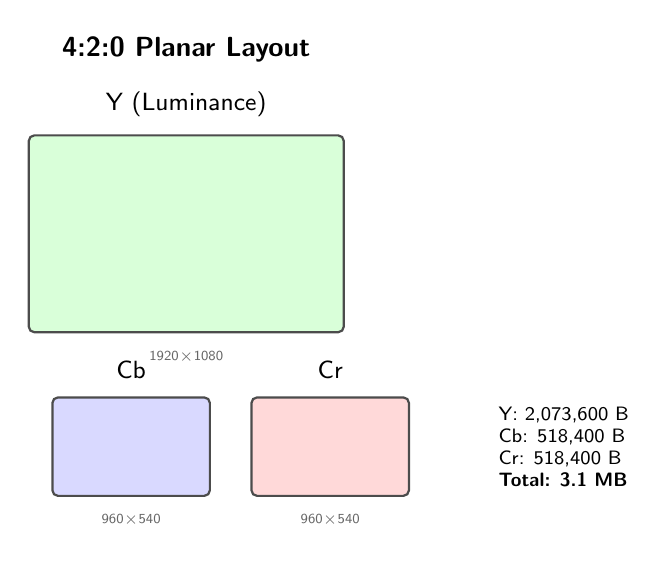
\begin{tikzpicture}[
    plane/.style={draw=black!70, thick, minimum width=4cm, minimum height=2.5cm, rounded corners=2pt},
    yplane/.style={plane, fill=green!15},
    cbplane/.style={plane, fill=blue!15, minimum width=2cm, minimum height=1.25cm},
    crplane/.style={plane, fill=red!15, minimum width=2cm, minimum height=1.25cm},
    label/.style={font=\small\sffamily},
    size/.style={font=\tiny\sffamily, text=black!60}
]

% Y plane
\node[yplane] (y) {};
\node[above=0.1cm of y, label] {Y (Luminance)};
\node[below=0.1cm of y, size] {1920$\times$1080};

% Cb plane
\node[cbplane, below right=0.8cm and 0.3cm of y.south west] (cb) {};
\node[above=0.1cm of cb, label] {Cb};
\node[below=0.1cm of cb, size] {960$\times$540};

% Cr plane
\node[crplane, right=0.5cm of cb] (cr) {};
\node[above=0.1cm of cr, label] {Cr};
\node[below=0.1cm of cr, size] {960$\times$540};

% Sizes annotation
\node[right=1cm of cr, align=left, font=\scriptsize\sffamily] {
    Y: 2,073,600 B\\
    Cb: 518,400 B\\
    Cr: 518,400 B\\
    \textbf{Total: 3.1 MB}
};

% Title
\node[above=0.8cm of y, font=\sffamily\bfseries] {4:2:0 Planar Layout};

\end{tikzpicture}
\end{document}
